\label{appendix_schematics}

All schematics in this Appendix were generated using gschem from the gEDA 
toolsuite.

These are all available in our GitHub repository \cite{github}, under the 
schematics/ folder. PDF and PS files are also available in the 
schematics/images folder.

Note that you need to run 
\begin{verbatim} 
$ gschem SCHEMATIC_NAME
\end{verbatim}
from within this folder to use the non-standard symbols available in that 
folder.

\section{Dummy Payload}
\begin{figure}[H]
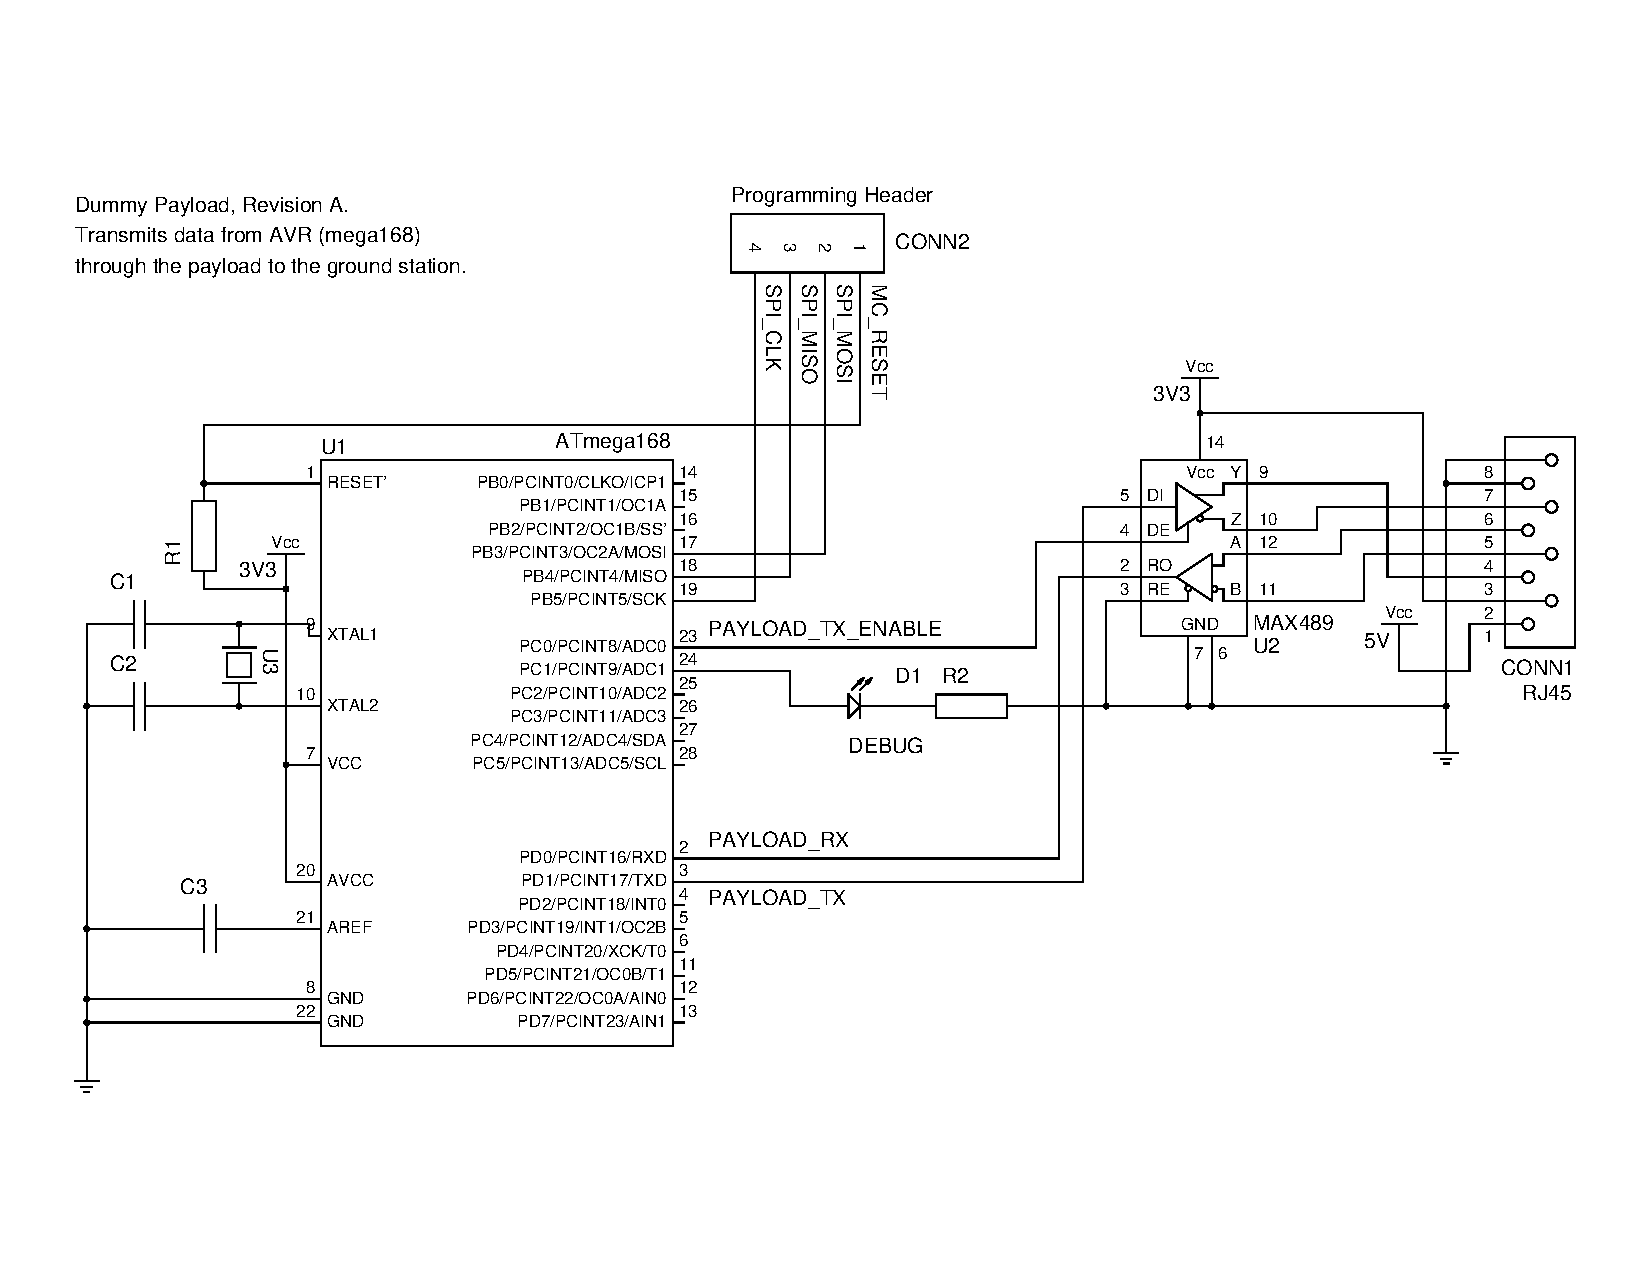
\includegraphics[width=1.4\textwidth, angle=90]{schematics/dummy_payload.pdf}
\caption{Schematic of the circuit used to test communication from a "dummy" 
payload to the autopilot module. Largely based on a schematic provided by 
our customer, and runs a slightly modified version of source code provided 
again, by our customer.}
\end{figure}

\section{Final Payload Module}
\label{Payload_Schematic}
\begin{figure}[H]
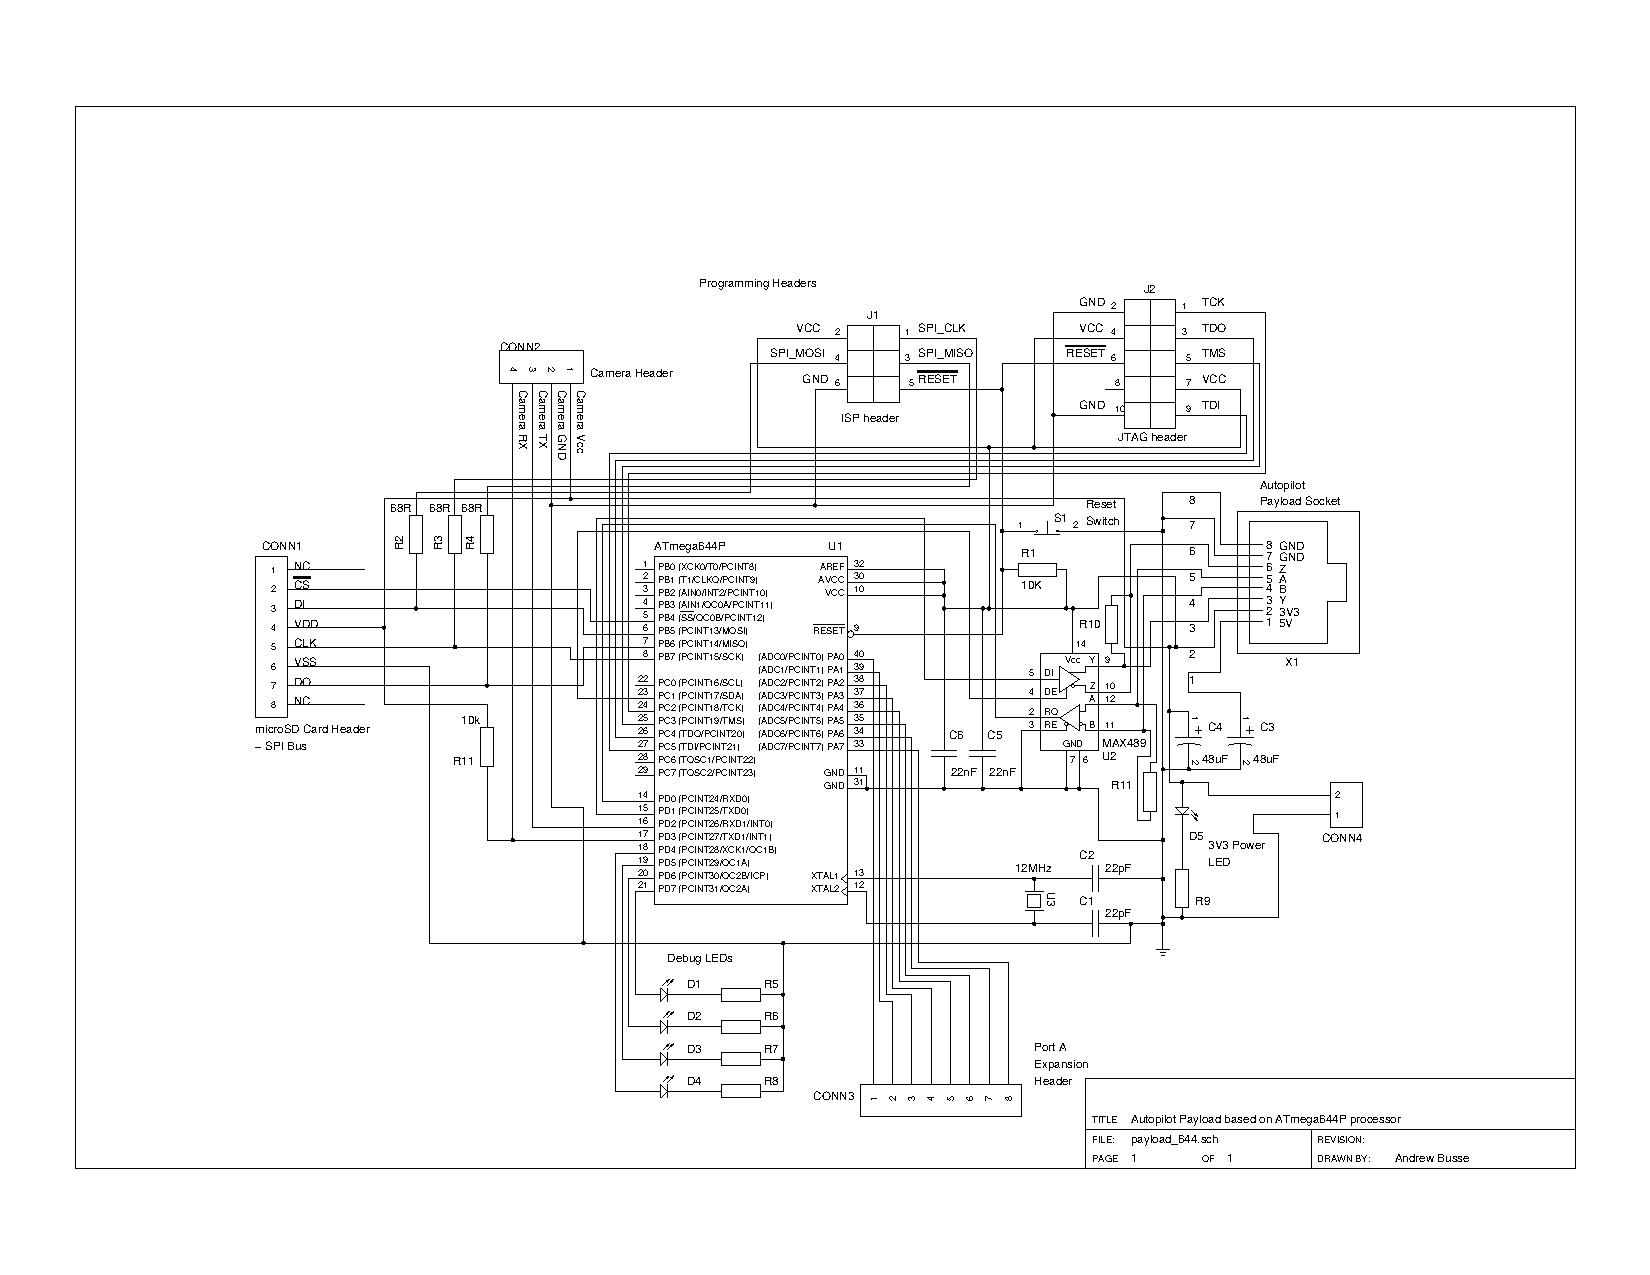
\includegraphics[width=1.4\textwidth, angle=90]{schematics/payload_644.pdf}
\caption{Final Schematic of the implemented payload module. See ??? for a 
detailed explanation of which components are for what purpose}
\end{figure}

\section{Payload: Arduino Uno with additional ATmega168}
\begin{figure}[H]
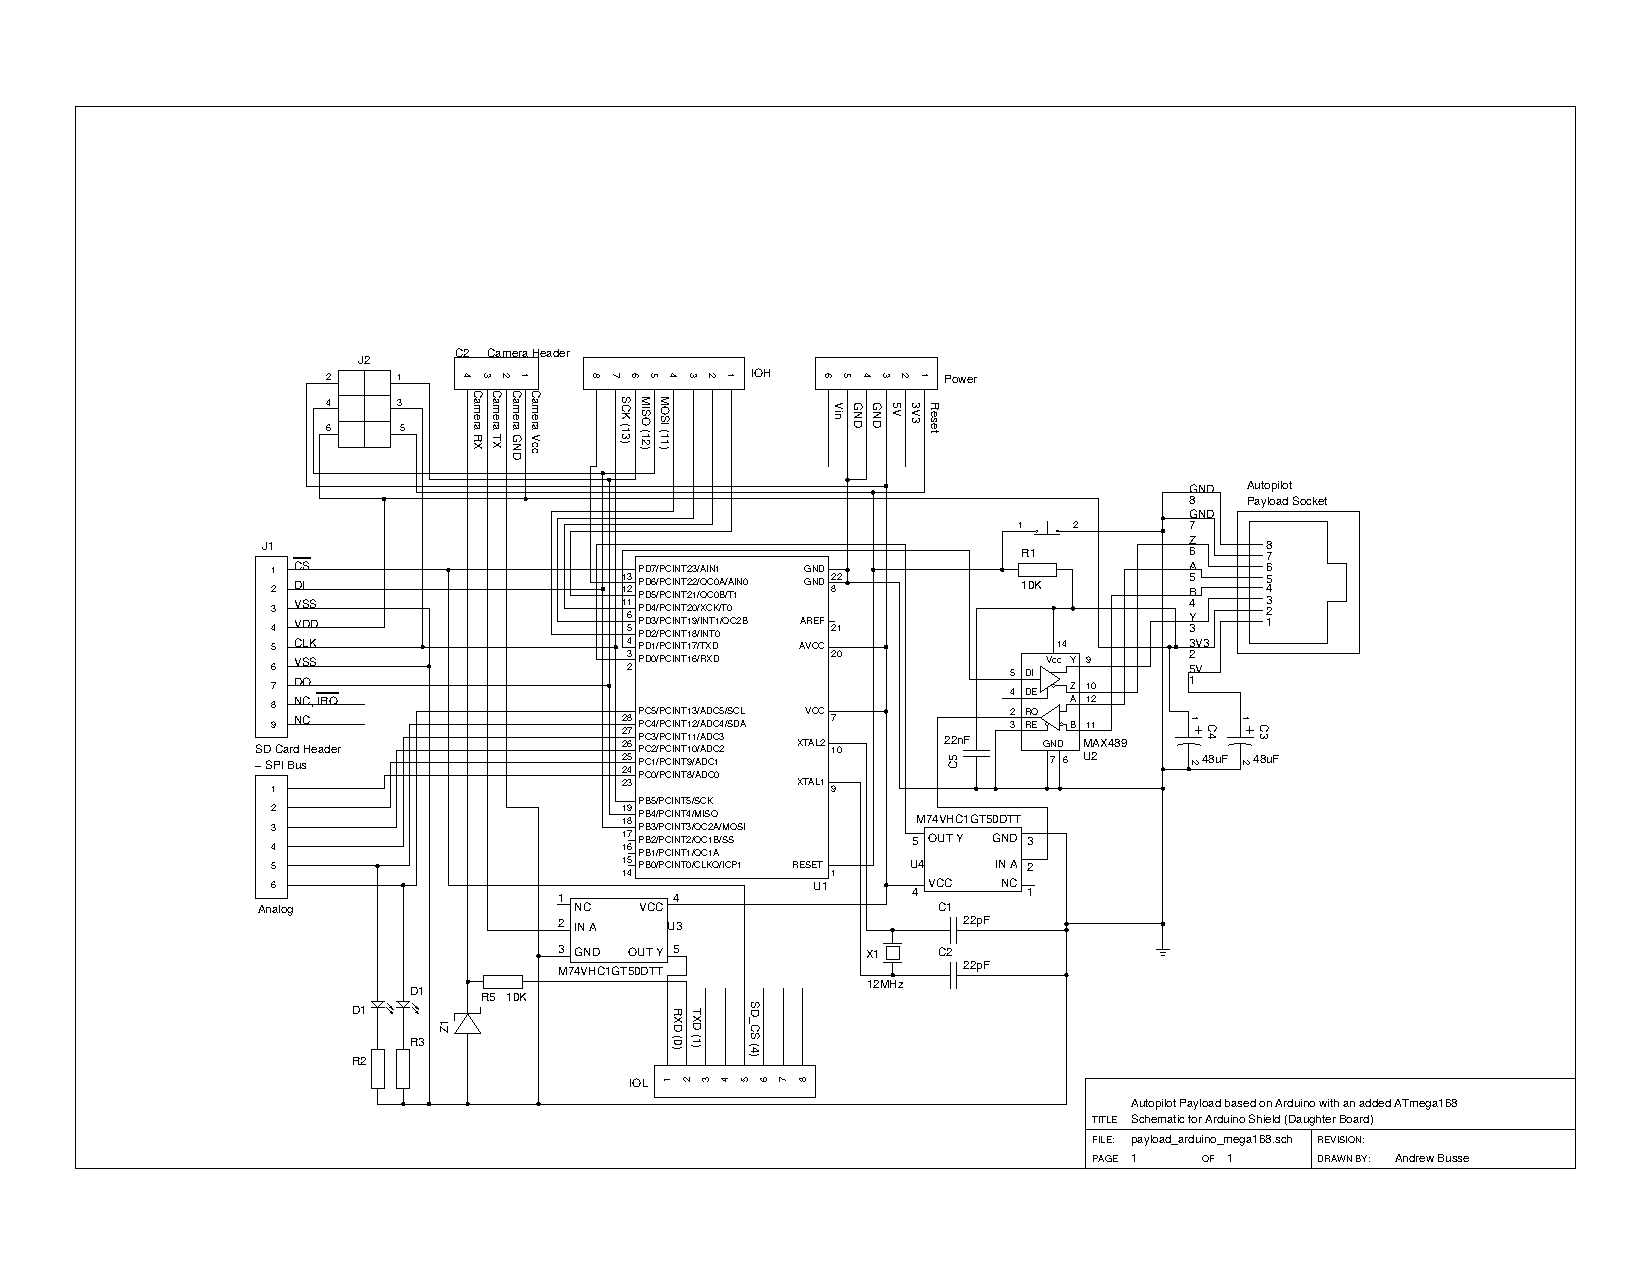
\includegraphics[width=1.4\textwidth, angle=90]{schematics/payload_arduino_mega168.pdf}
\caption{Schematic for a considered payload module ???reference???: an 
Arduino Uno with a daughter board containing an ATmega168 for Autopilot to 
Payload module communication.}
\end{figure}

\section{Payload: Arduino Uno with Multiplexed UART line}
\begin{figure}[H]
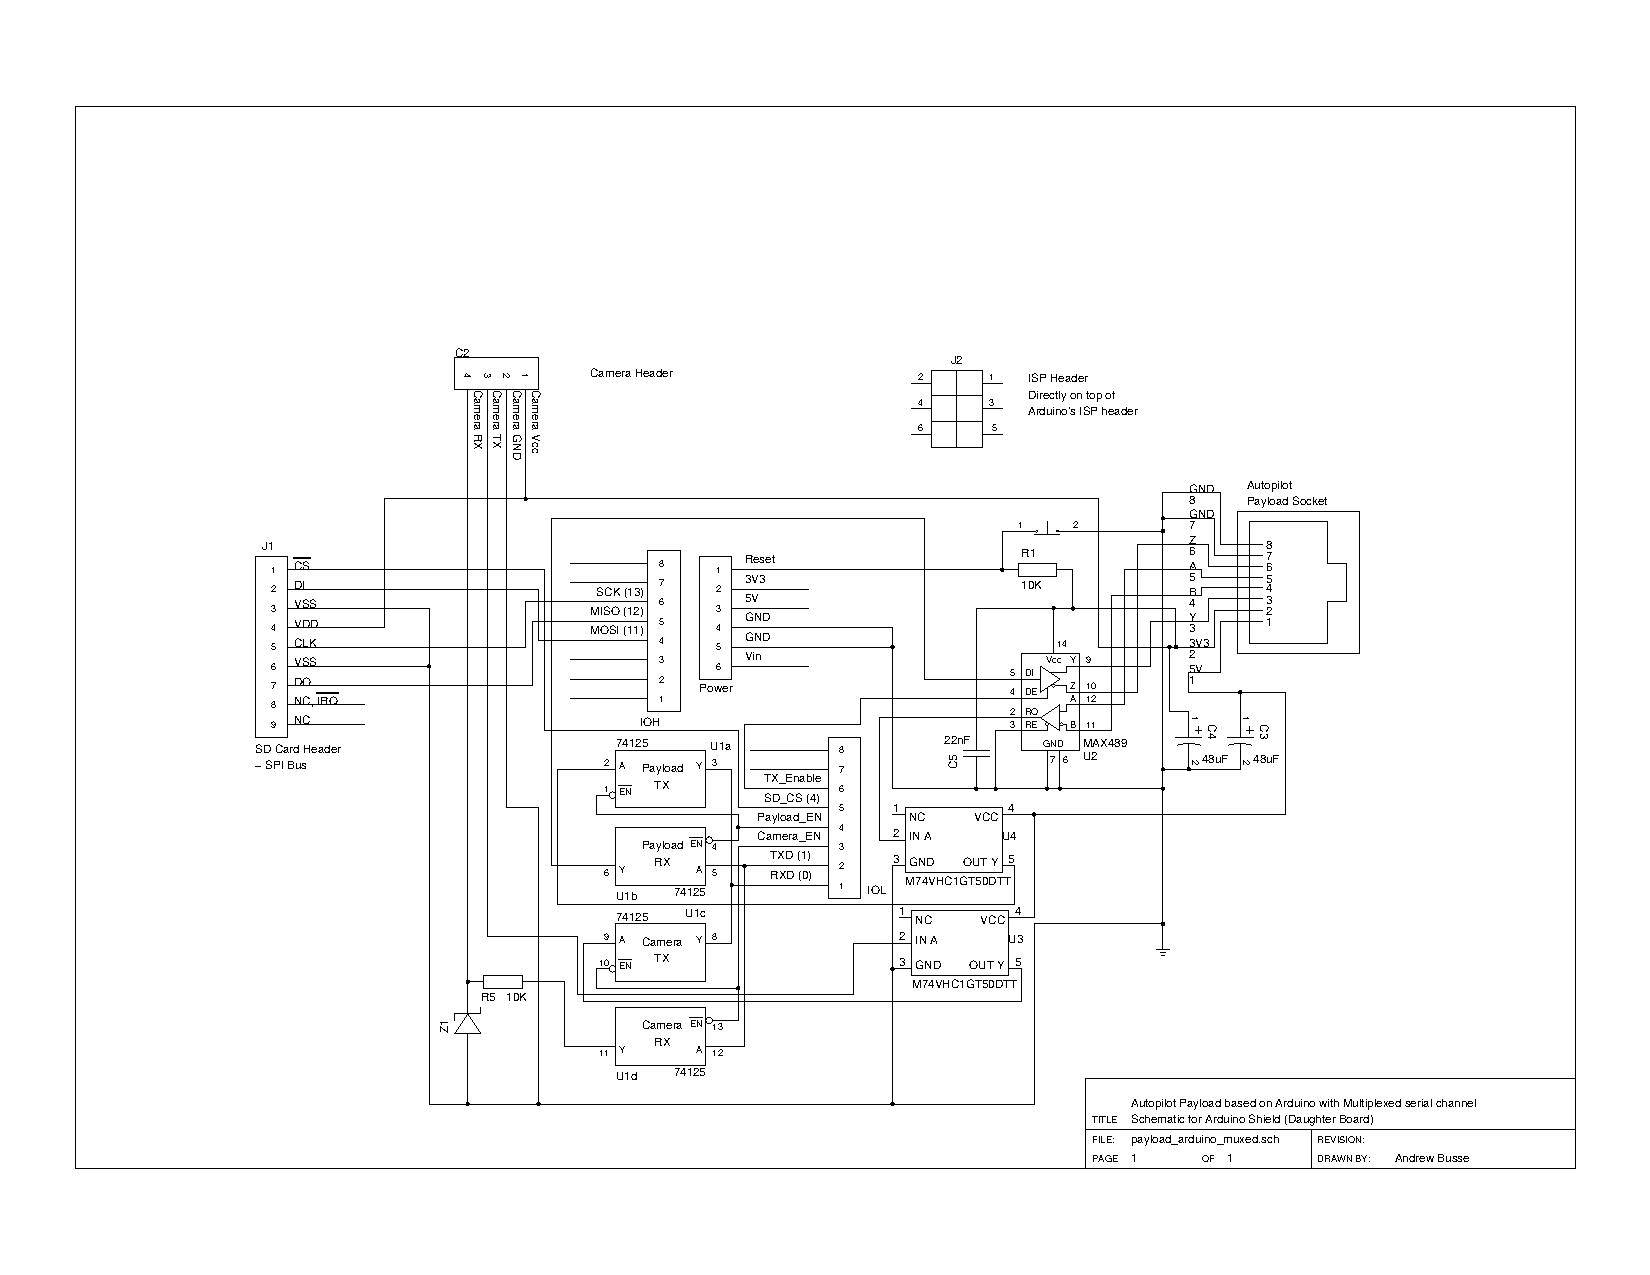
\includegraphics[width=1.4\textwidth, angle=90]{schematics/payload_arduino_muxed.pdf}
\caption{Schematic for a considered payload module ???reference???: an 
Arduino Uno with its UART line multiplexed between camera and autopilot 
communication}
\end{figure}
